\documentclass[12pt, a4paper]{article}
\usepackage{graphicx}
\usepackage{amsmath}
\usepackage{float}

\title{
    EE2703: Applied Programming Lab \\
    \Large Assignment 3: Linear Least Squares Fitting
}

\author{Soham Roy \\ \normalsize EE20B130}

\date{\today}

\begin{document}

\maketitle % Insert the title, author and date


\section{Introduction}
For this assignment we use the Bessel function and Gaussian noise to study
the effect of changing standard deviation on the linear fitting of the data.
\begin{equation*}
    f(t) = AJ_2(t) + Bt + n(t)
\end{equation*}
Where, $A = 1.05$, $B = -0.105$, $J_2 =$ Bessel function, $n(t) =$ Noise function.
Our aim is to relate the error in estimating $A$, $B$ to the
standard deviation of the Gaussian noise.


\section{Subquestions}
\subsection{Generate the Data}
On running the python script \texttt{generate\_data.py}, the data is written to
the file \texttt{fitting.dat}. The \texttt{scipy} library has been used to calculate
the Bessel function. The \texttt{numpy.array t} contains 101 equally spaced numbers
between 0 and 10, which are fed into the Bessel function and added with noise to
generate the data.


\subsection{Load the Data}
The data from \texttt{fitting.dat} is loaded using \texttt{numpy.loadtxt()}.
The first column of \texttt{raw\_data} are the time values, and the subsequent
columns are the corresponding noisy data values.
\begin{verbatim}
    raw_data = loadtxt(DATAFILE)

    Time = raw_data[:, 0]
    F = raw_data[:, 1:]
\end{verbatim}


\subsection{The Function and the Noise}
The true values are generated using \texttt{F\_true = g(Time)},
where the function \texttt{g(t,A,B)} defined as:
\begin{verbatim}
    def g(t, A=A_true, B=B_true):
        return A * jn(2, t) + B * t
\end{verbatim}
where \texttt{A\_true, B\_true = 1.05, -0.105} are the true values of $A$ and $B$. \\
The noise is generated using \texttt{Sigma = logspace(-1, -3, K)}, where
\texttt{K = 9} is the number of curves to be plotted.


\subsection{Plot the Data}
We plot the data along with the function \texttt{g(t,A,B)} for
\texttt{A=1.05}, \texttt{B=-0.105}.
\begin{verbatim}
    plot(Time, F)
    plot(Time, F_true, color='black', lw=2)
\end{verbatim}
\begin{figure}[H]
    \centering
    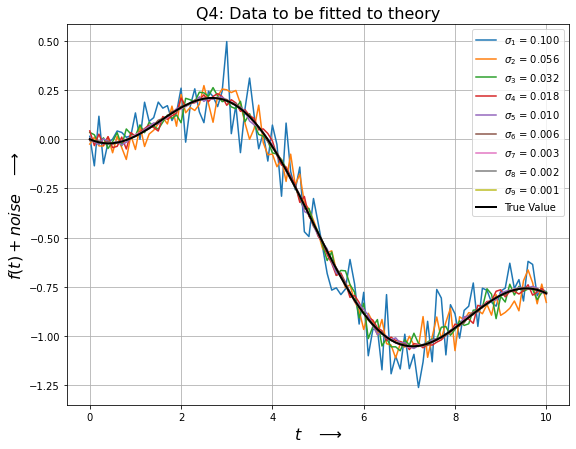
\includegraphics[scale=0.6]{Q4.png}
\end{figure}


\subsection{Plot with Error Bars}
A plot of the first column of data with error bars has been generated, with every
$5^{th}$ data item plotted for readability. The exact curve has also been plotted
to see how much the data diverges.
\begin{verbatim}
    errorbar(Time[::5], F[::5, 0], Sigma[0], fmt="ro")
    plot(Time, F_true, color='black', lw=2)
\end{verbatim}
\begin{figure}[H]
    \centering
    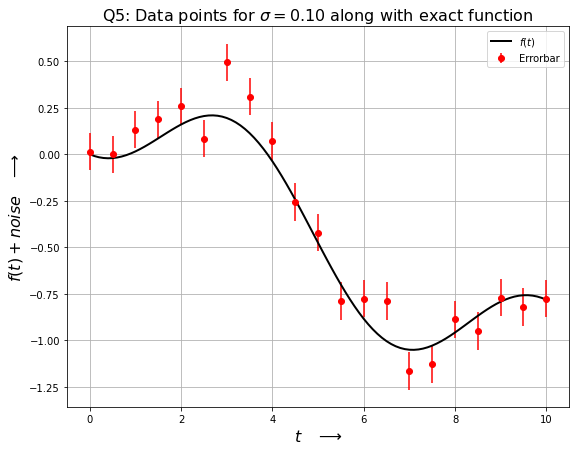
\includegraphics[scale=0.6]{Q5.png}
\end{figure}


\subsection{Equate the Vectors}
\begin{gather}
    g(t,A,B) =
    \begin{pmatrix}
        J_2(t_1) & t_1   \\
        \dots    & \dots \\
        J_2(t_m) & t_m
    \end{pmatrix}
    \begin{pmatrix}
        A \\ B
    \end{pmatrix}
    \equiv
    M \cdot P
    \label{eq:M}
\end{gather}
\texttt{F\_true.reshape(N, 1)} is $g(t,A,B)$, the vector of the true values. \\
\texttt{M = c\_[jn(2, Time), Time]} generates $M$, which is multiplied by \\
\texttt{[[A\_true], [B\_true]]}, i.e. $P$, to obtain the RHS vector.\\
\texttt{assert} ensures that the two vectors are equal by evaluating \\
\texttt{numpy.allclose()}, as we cannot reliably equate floats.


\subsection{Mean Squared Error}
The mean squared error between the data ($f_k$) and the assumed model has been
calcuated for every combination of $A$ and $B$, where $A$ and $B$ range from 0 to 1
and -0.2 to 0 respectively. \\
The following formula has been implemented:
\begin{equation*}
    \epsilon_{ij} = \frac{1}{101} \sum_{k=0}^{101} (f_k - g(t_k, A_i, B_j))^2
\end{equation*}
by looping over the following line of code:
\begin{verbatim}
    eps[i][j] = mean((F[:, 0] - g(Time, A[i], B[j])) ** 2)
\end{verbatim}


\subsection{Plot the MSE}
The contour plot has been generated by \texttt{contour}, and labeled using
\texttt{clabel}. Further, the exact location of \texttt{(A\_true, B\_true)} has been
plotted and annotated.
\begin{verbatim}
    clabel(contour(A, B, eps, 15))
    plot([A_true], [B_true], "ro")
    annotate("Exact location", xy=(A_true, B_true), size=16)
\end{verbatim}
\begin{figure}[H]
    \centering
    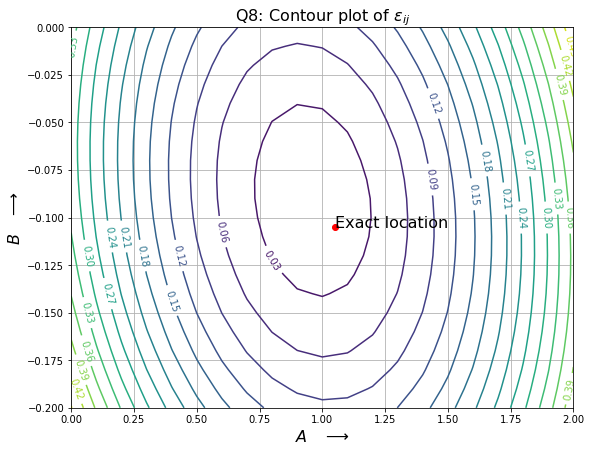
\includegraphics[scale=0.6]{Q8.png}
\end{figure}


\subsection{Best Estimate for A and B}
The matrix $M$, defined in Equation \ref{eq:M}, has been used to find the best estimate
of $A$ and $B$ for the first column of data. This was done by computing the
least-squares solution for it using \texttt{scipy.linalg.lstsq()} to print:
\begin{verbatim}
"Best estimate:   A = {}, B = {}".format(*lstsq(M, F[:, 0])[0])
\end{verbatim}


\subsection{Plot the Errors in A, B}
The errors in $A$ and $B$ have been calculated by subtracting the true values:
\begin{verbatim}
    Aerr, Berr = abs(lstsq(M, F)[0] - [[A_true], [B_true]])
\end{verbatim}
These have thus been plotted against the standard deviations of the data:
\begin{verbatim}
    plot(Sigma, Aerr, 'o', linestyle="dashed")
    plot(Sigma, Berr, 'o', linestyle="dashed")
\end{verbatim}
\begin{figure}[H]
    \centering
    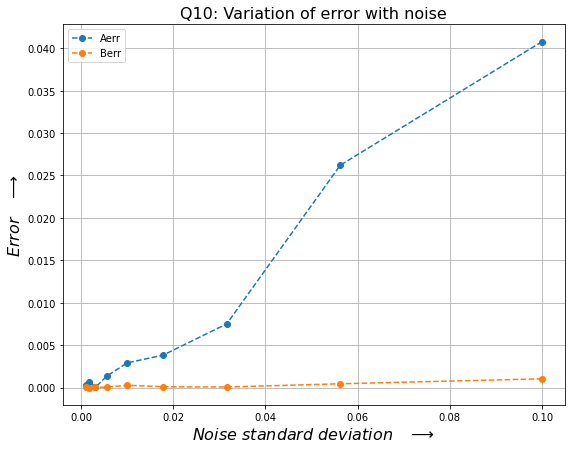
\includegraphics[scale=0.6]{Q10.png}
\end{figure}
\pagebreak


\subsection{Plot using log-log Scale}
The scale of the graph has been changed to log-log, with an \texttt{errorbar()} plot:
\begin{verbatim}
    xscale("log")
    yscale("log")
    errorbar(Sigma, Aerr, Sigma, fmt="o")
    errorbar(Sigma, Berr, Sigma, fmt="o")
\end{verbatim}
\begin{figure}[H]
    \centering
    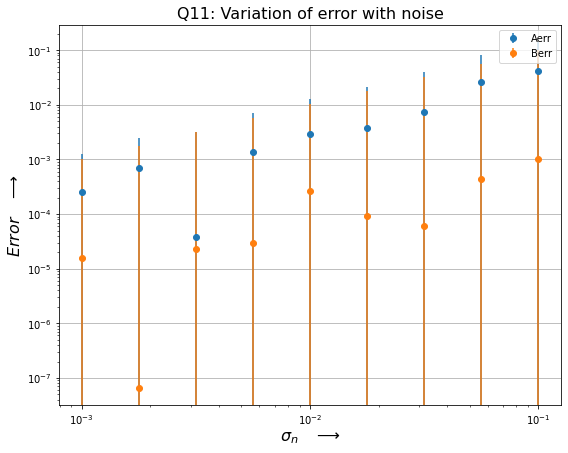
\includegraphics[scale=0.6]{Q11.png}
\end{figure}


\section{Conclusion}
As we see from the plots, the error in estimated $A$ and $B$ increases with increase in
the standard deviation of the Gaussian noise in the data. Further, we see that the
increase is somewhat linear when plotted on a log-log scale.


\end{document}
